\chapter{Ensayos y resultados}
\label{Chapter4}
En este capítulo se describen los ensayos realizados y los resultados obtenidos en el desarrollo del sistema de detección del picudo rojo. Se detallan las etapas de preparación del dataset, el entrenamiento de los modelos de detección, la integración de los modelos en la aplicación web y finalmente los resultados obtenidos en producción.

%----------------------------------------------------------------------------------------
%	SECTION 1
%----------------------------------------------------------------------------------------
\section{Preparación y organización del entrenamiento}
\label{sec:preparacionDataset}

Debido a la gestión de la infraestructura realizada en etapas anteriores (referirse al capítulo \ref{Chapter3}), se pudo contar con un dataset de imágenes aéreas etiquetadas para entrenar el modelo de detección. La estructura de entrenamiento se basó en la plantilla de \textit{cookiecutter data science}, que permite organizar los datos y scripts de manera eficiente y reproducible. En esta plantilla se define la siguiente estructura de directorios adaptada a este proyecto:

\begin{lstlisting}[label=cod:vControl,caption=Estructura de directorios utilizada., literate={├}{{\textSFviii}}1 {─}{{\textSFx}}1 {└}{{\textSFii}}1 {│}{{\textSFxi}}1]  % Start your code-block

modulo-IA
├── data
│   ├── iterim
│   ├── processed
│   │   ├── yolo_palm_detection_datset_v1.0
│   │   └── yolo_rpw_detection_dataset_v1.0
│   ├── raw
│   │   └── coco_palm_dataset_v1.0
│   └── temp
├── models
│   ├── coco_palm_detection_yolo11n_640.pt
│   ├── coco_palm_detection_yolo11x_640.pt
│   ├── coco_rpw_detection_yolo11n_640.pt
│   └── coco_rpw_detection_yolo11x_640.pt
└── modulo_ia
    ├── modeling
    ├── utils
    ├── config.py
    ├── dataset.py
    ├── features.py
    └── main.py
notebooks
├── deteccion_palmeras
│   └── yolovll
│       └── 3.01-bm-deteccion-palmeras-yolov11.ipynb
└── deteccion_picudo_rojo
    └── yolov11
        └── 3.02-bm-deteccion-rpw-yolov11.ipynb
poetry.lock
pyproject.toml

\end{lstlisting}

El dataset se organizó en dos directorios:
\begin{itemize}
    \item \textit{Raw dataset}: contiene las imágenes originales sin procesar, junto con sus anotaciones en formato COCO. Estas imágenes fueron descargadas desde el almacenamiento en la nube (MinIO) y representan el conjunto completo de datos disponibles para el entrenamiento. Se descargaron aquellas imágenes que contenían detecciones, lo que resultó en un total de 892 imágenes etiquetadas, en donde se presentan 5.670 instancias de palmeras sanas, 57 instancias de palmeras infectadas, 40 exterminadas y 110 instancias de palmeras muertas.
    \item \textit{Processed dataset}: contiene las imágenes procesadas y preparadas para el entrenamiento del modelo. Son imágenes que son directamente consumidas por el modelo para el entrenamiento y validación.
\end{itemize}

Esta organización recomendada por \textit{cookiecutter data science} permite mantener un flujo de trabajo claro y estructurado, en donde el \textit{raw dataset} permanece inalterado, mientras que el processed dataset puede ser modificado y ajustado según las necesidades del entrenamiento. El directorio \textit{interim} se utiliza para almacenar datos intermedios generados durante el procesamiento del dataset final, y el directorio temp se emplea para datos temporales que no necesitan ser versionados. En este caso, no se guardó los datos intermedios ni temporales, por lo que ambos directorios permanecen vacíos. La descarga del dataset se realizó utilizando scripts de Python que interactúan con la API de MinIO para obtener las imágenes, sus correspondientes anotaciones de la base de datos y finalmente la conversión al formato COCO. La clase \lstinline[language=sh]|dataset.py| centraliza todas estas funcionalidades.

El procesamiento del dataset final incluyó dos conjuntos que pasaron por varias etapas, como la conversión de las anotaciones al formato YOLO, el recorte de las imágenes en sub-imágenes más pequeñas para mejorar la detección utilizando SAHI\footnote{Método en donde se divide una imagen en varias imágenes más pequeñas.}, el balanceo del dataset para abordar la desproporción entre las clases y la creación de los splits de entrenamiento, validación y prueba. Se utilizó la herramienta FiftyOne para la visualización y validación del dataset, así como obtener las métricas de calidad. Un resumen de las operaciones aplicadas al dataset y sus directorios de salida se presenta en la tabla \ref{tab:procesamiento-dataset}.

\begin{table}[H]
    \centering
    \caption{Resumen de las operaciones aplicadas al dataset durante el procesamiento.}
    \label{tab:procesamiento-dataset}
    \begin{tabular}{ l l l}
        \toprule
        \textbf{Etapa}                                 & \textbf{Directorio de salida} \\ \hline
        \midrule
        Dataset original (COCO)                        & Raw                           \\ \hline
        Conversión a formato YOLO                      & Interim                       \\ \hline
        Recortes de \SI{640}{}\,\texttimes\,\SI{640}{} & Interim                       \\ \hline
        Balanceo de clases                             & Interim                       \\ \hline
        Splits finales (80\%/10\%/10\%)                & Processed                     \\ \hline
        \bottomrule
        \hline
    \end{tabular}
\end{table}

Dentro de las etapas, se destaca el recorte de las imágenes utilizando SAHI, que demora usualmente cerca de 20 minutos en procesarse y el balanceo del dataset, en donde se decidió simplemente aplicar \textit{undersampling} \citep{noauthor_oversampling_2025}, en donde se reduce la cantidad de detecciones de las clases mayoritarias (palmeras sanas) para igualar la cantidad de detecciones de las clases minoritarias (palmeras infectadas, exterminadas y muertas). Esta decisión se tomó debido a la poca cantidad de datos disponibles para las clases minoritarias, lo que dificultaba la aplicación de técnicas de \textit{oversampling} sin incurrir en un sobreajuste significativo.

% Hablar de la descarga de las imágenes de MinIO, en formato coco.
% Hablar de la organización de las carpetas (cookiecutter data science).
% Hablar del pipeline de datos:
% - Cantidad de datos del raw-dataset.
% - Procesamiento del dataset (convertir a una clase, convertir a formato YOLO, recortar en imágenes pequeñas para SAHI, balancear el dataset, splits finales).
% Hablar de la cantidad de datos del processed-dataset.
% Hablar de las herramientas utilizadas (principalmente FiftyOne).
% Validaciones y muestreo de algún batch de imágenes.

%----------------------------------------------------------------------------------------
%	SECTION 2
%----------------------------------------------------------------------------------------
\section{Entrenamiento y resultados de modelos}
\label{sec:entrenamientoModelos}

% Hablar de la decision de utilizar Yolov11.
% Hablar de la decisión de entrenar dos modelos (palmeras y picudo rojo).
% Hablar del fine-tuning del modelo 
% Tarjeta de video utilizada.

Debido a la naturaleza del problema y a la poca cantidad de datos de las clases más importantes, se optó por realizar un entrenamiento de dos modelos: uno para la detección de palmeras y otro para la detección del picudo rojo. En base a la literatura estudiada (referirse a la sección \ref{sec:estadoArte}), se sabía que modelos de la familia Yolo habían demostrado un buen desempeño en tareas de detección de palmeras en imágenes areas. Por lo tanto, se decidió utilizar YoloV11 (el modelo más actual de la familia Yolo hasta el momento de ejecución de los entrenamientos) como arquitectura base para ambos modelos. Esta versión tiene una mejora en performance y tiempo de procesamiento con respecto a versiones anteriores, como se puede apreciar en la figura \ref{fig:yolov11-comparison}.

\begin{figure}[H]
    \centering
    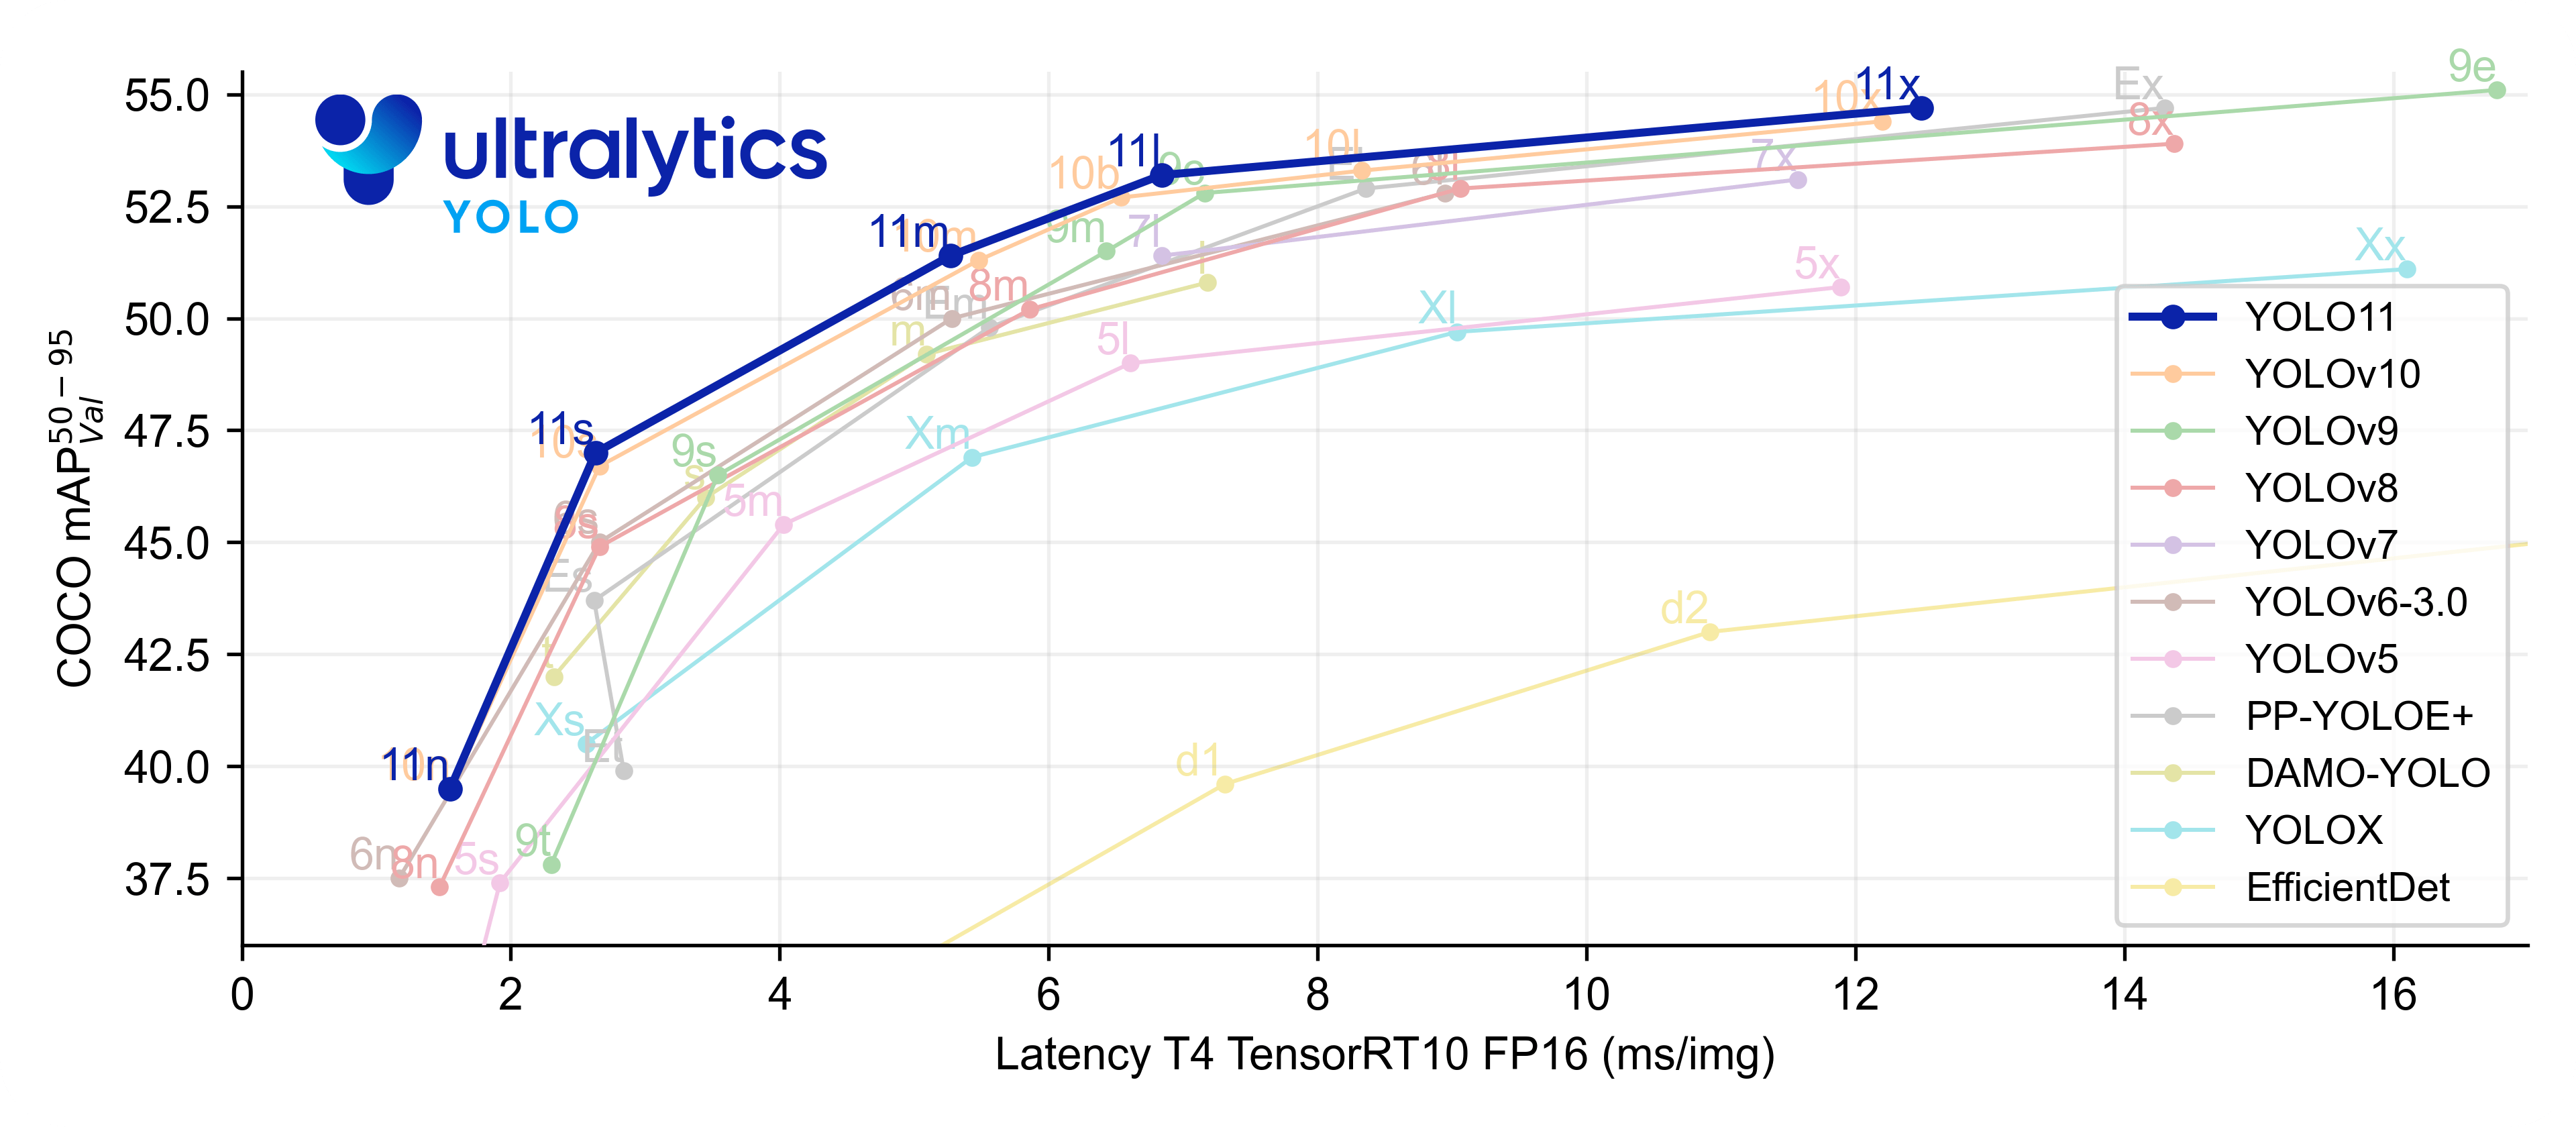
\includegraphics[scale=0.1]{./Figures/performance-comparison-yolov11.png}
    \caption{Comparación de performance entre YoloV11 y versiones anteriores. \protect\footnotemark}
    \label{fig:yolov11-comparison}
\end{figure}

\footnotetext{ Imagen obtenida de \url{https://docs.ultralytics.com/es/models/yolo11/}}

Se esperaba alcanzar un mAP superior al 0.85 (mAP50) para la detección de palmeras, según evidencia actual, principalmente en el artículo de N. Najiv Zhorif et al \citep{zhorif_implementation_2024}, donde se logró un mAP de cerca del 0.85 utilizando Yolov8 y SAHI \citep{akyon_slicing_2022}, con imágenes de resoluciones similares.

El enfoque del entrenamiento se centró en el fine-tuning de modelos yolo (en su versión nano y su versión extra grande) preentrenados en el dataset COCO, utilizando \textit{transfer learning} \citep{jacob_murel_phd_what_2024} para adaptar los modelos a la tarea específica de detección de palmeras. Luego, este modelo se utilizó como base para el entrenamiento del modelo de detección del picudo rojo, aplicando nuevamente \textit{transfer learning}, con diferencia que en este caso se congeló durante las primeras épocas las capas iniciales del modelo (técnica obtenida de Yosinski et al. \citep{yosinski_how_2014} y Goodfellow et al. \footnote{ Capítulo 15: \textit{Representation Learning}} \citep{goodfellow_deep_2016} ). Este enfoque puede visualizarse en la figura \ref{fig:training-learning}.

% TODO: Poner imagen del pipeline de procesamiento del dataset con los datos de las imágenes intermedias.
\begin{figure}[H]
    \centering
    
\includegraphics[scale=0.5]{./Figures/place-holder.png}
    \caption{Esquema del enfoque de entrenamiento basado en \textit{transfer learning}.}
    \label{fig:training-learning}
\end{figure}

El entrenamiento se realizó utilizando una tarjeta gráfica NVIDIA GeForce RTX 4080 SUPER, que cuenta con 16 GB de memoria GDDR6X, lo que permitió manejar los modelos y datasets sin problemas de memoria. Se utilizaron las librerías Ultralytics y PyTorch para la implementación y entrenamiento de los modelos. Los hiperparámetros se ajustaron mediante experimentación, buscando un equilibrio entre la tasa de aprendizaje, el tamaño del batch y el número de épocas para evitar el sobreajuste.
Un resumen hardware utilizado para el entrenamiento se presenta en la tabla \ref{tab:hardware-entrenamiento}.

\begin{table}[H]
\centering
\caption{Resumen del hardware utilizado para el entrenamiento de los modelos.}
\label{tab:hardware-entrenamiento}
\begin{tabular}{ l l }
    \toprule
    \textbf{Componente} & \textbf{Especificación}                      \\ \hline
    \midrule
    GPU                 & NVIDIA GeForce RTX 4080 SUPER (16 GB GDDR6X) \\ \hline
    CPU                 & Intel Core i7-12700KF (12 núcleos)           \\ \hline
    RAM                 & 128 GB DDR5 (5600 MHz)                       \\ \hline
    Almacenamiento      & SSD NVMe 1 TB                                \\ \hline
    Sistema Operativo   & Windows 11                                   \\ \hline
    \bottomrule
    \hline
\end{tabular}

\subsection{Detección de palmeras}
\label{sec:deteccionPalmeras}


% Hablar de los tamaños de los
% Hablar de los experimentos realizados.
% Hablar de los hiperparámetros utilizados.
% Hablar del aumento de datos.
% Hablar de los resultados obtenidos.
% Hablar de las herramientas utilizadas (FiftyOne, Supervision).
% Graficas:
% - Curvas de entrenamiento (loss, mAP, precision, recall).
% - Curvas de validación (mAP, precision, recall).
% - Matriz de confusión.
% Hablar de las validaciones realizadas (matriz de confusión, mAP, precision, recall, F1-score).

\subsection{Detección del picudo rojo}
\label{sec:deteccionPicudo}

% TODO: Poner imagen del pipeline de procesamiento del dataset con los datos de las imágenes intermedias.


% Hablar de los tamaños de los
% Hablar de los experimentos realizados.
% Hablar de los hiperparámetros utilizados.
% Hablar del aumento de datos.
% Hablar de los resultados obtenidos.
% Hablar de las herramientas utilizadas (FiftyOne, Supervision).
% Graficas:
% - Curvas de entrenamiento (loss, mAP, precision, recall).
% - Curvas de validación (mAP, precision, recall).
% - Matriz de confusión.
% Hablar de las validaciones realizadas (matriz de confusión, mAP, precision, recall, F1-score).
% Hablar de la función de pérdida de YoloV11 (como se le dió más importancia a las clases).

%----------------------------------------------------------------------------------------
%	SECTION 3
%----------------------------------------------------------------------------------------

\section{Integración del modelo en la aplicación web}
\label{sec:integracionModelo}

% Hablar del proceso de despliegue de los modelos.
% Hablar de las herramientas utilizadas para el despliegue de los modelos.
% Hablar de los problemas encontrados y como se resolvieron.
% Hablar del modelo de detección de palmeras y el de detección de picudo rojo.
% Hablar de la integración con la aplicación web.
% Hablar del empaquetamiento del modelo (con Poetry).


%----------------------------------------------------------------------------------------
%	SECTION 4
%----------------------------------------------------------------------------------------
\section{Resultados en producción}
\label{sec:resultadosProducción}

% Hablar de los resultados obtenidos en producción con nuevos vuelos de drones.
% Hablar del uso de la aplicación web por parte de los usuarios finales.
% Hablar de los tiempos de predicción y la escalabilidad del sistema.
% Hablar de los thresholds utilizados para la detección de palmeras y picudo rojo.
% Hablar de los requerimientos de la app.
